\documentclass{article}
\usepackage{geometry}
\geometry{a4paper}
\usepackage{ctex}%中文
\usepackage{graphicx}%图片
\usepackage{multirow}%表格
\usepackage{amsmath}%公式,公式换行等时候会用到
\usepackage{amsmath}
\usepackage{amsfonts}%特殊符号,比如说实数集
\usepackage{subfigure} 
\title{最优化学习笔记2(p23-p)}
\author{BD S}
\begin{document}
\maketitle
\tableofcontents


\newpage
本章将从范数和导数讲起,接着介绍广义实值函数、凸集、凸函数、共轭函数和次梯度等凸分析方面的概念以及结论
%%%%%%%%%%%%%%%%%%%%%%%%%%%%%%%%%%%%%%%%%%%%%%%%%%%%%%%%%%%%%%%%%%%%%%%%%%%%%%%%%%%%%%%%%%%%%%%%%%%%%%%%%%%%%%%%%%%%%%%%%%%%%%%%%%%%%%%%%%%%%%%%%%%%%%%%%%%%%%%%%%%%%%%%%%%%%%%%%%%%%%%%%%%%%%%%%%%%%%%%%%%%%%%%%%%%%%%%%%%%%%%%%%%%%%%%%%%%%%%%%%%%%%
\section{范数}
\subsection{向量范数}

首先是范数的定义
\newtheorem{definition}{Definition}
\begin{definition}
    从向量空间$\mathbb{R}^n$到实数域$R$的非负函数$||\cdot||$,满足正定性、齐次性、三角不等式,那么它就是范数
\end{definition}

$l_p$范数:$$||v||_p=(|v_1|^p+|v_2|^p+...+|v_n|^p)^{\frac{1}{p}}$$
当$p=0$时候,$l_0$范数就是非0元素个数,当$p=1$时候,$l_1$范数就是绝对值之和,当$p=2$时候,$l_0$范数就是平方和开根,当$p=\infty$时候,$l_0$范数就是元素的最大值。
\subsection{矩阵范数}
矩阵的$l_1$范数就是所有的元素之和,$||A||_1=\sum\limits_{i=1}^m\sum\limits_{j=1}^n|a_{ij}|$,矩阵的$l_2$范数也就是矩阵的$F$范数。就是所有元素的平方和开根。
常用的范数还有核范数,为所有非0奇异值之和。给定矩阵$A \in \mathbb{R}^{m \times n}$,核范数定义为$$||A||_*=\sum\limits_{i=1}^r \sigma_i,\ i=1,2,\dots,r $$,并且$r$是矩阵的秩。
\subsection{矩阵内积}
Frobenius内积:$$<A,B>\overset{def}{=}Tr(AB^T)=\sum\limits_{i=1}^m\sum\limits_{j=1}^na_{ij}b_{ij}$$对应的也有矩阵范数的柯西不等式$$|<A,B>| \le ||A||_F ||B||_F$$等号在$A$和$B$线性相关的时候成立。
%%%%%%%%%%%%%%%%%%%%%%%%%%%%%%%%%%%%%%%%%%%%%%%%%%%%%%%%%%%%%%%%%%%%%%%%%%%%%%%%%%%%%%%%%%%%%%%%%%%%%%%%%%%%%%%%%%%%%%%%%%%%%%%%%%%%%%%%%%%%%%%%%%%%%%%%%%%%%%%%%%%%%%%%%%%%%%%%%%%%%%%%%%%%%%%%%%%%%%%%%%%%%%%%%%%%%%%%%%%%%%%%%%%%%%%%%%%%%%%%%%%%%%
\section{导数}
\subsection{梯度与海瑟矩阵}
本章重点:梯度、海瑟矩阵、之间的关系以及雅可比矩阵。

当优化问题没有显式解的时候,可以通过函数值和导数信息来构造可以求解的子问题。首先是梯度的定义。
\begin{definition}
    定义一个函数$f:\mathbb{R}^n \rightarrow \mathbb{R}$,且$f$在点$x$的一个领域内有意义,若存在向量$g \in \mathbb{R}^n$满足$$\lim\limits_{p \rightarrow 0} \frac{f(x+p)-f(x)-g^Tp}{||p||}=0$$
    就称$f$在点$x$处可微,$g$成为$f$在点$x$处的梯度,记作$\bigtriangledown f(x)$。
\end{definition}

同时,如果$x$是一个向量,那么就有$$\bigtriangledown f(x) =[\frac{\partial f(x)}{\partial x_1},\frac{\partial f(x)}{\partial x_2},...,\frac{\partial f(x)}{\partial x_n}]^T$$
这是一阶偏导,还有二阶偏导(海瑟矩阵)
$$
    \bigtriangledown^2 f(x) =
    \left[
    \begin{array}{cccc}
        \frac{\partial^2 f(x)}{\partial x_1^2} &
        \frac{\partial^2 f(x)}{\partial x_1 \partial x_2} & 
        \dots &
        \frac{\partial^2 f(x)}{\partial x_1 \partial x_n }         \\
        \frac{\partial^2 f(x)}{\partial x_2 \partial x_1} &
        \frac{\partial^2 f(x)}{ \partial x_2^2} &
        \dots &
        \frac{\partial^2 f(x)}{\partial x_1 \partial x_n } \\
        \vdots &
        \vdots &
        \ddots &
        \vdots \\
        \frac{\partial^2 f(x)}{\partial x_n \partial x_1} &
        \frac{\partial^2 f(x)}{ \partial x_n \partial x_2} &
        \dots &
        \frac{\partial^2 f(x)}{\partial x_n^2} 
    \end{array}
    \right]
$$
二阶可微:$\bigtriangledown^2 f(x)$在区域$D$的每个$x$处都存在。如果还连续,就是二阶连续可微,且这个时候,海瑟矩阵对称。

接下来是雅可比矩阵。对于一个函数$f:\mathbb{R}^n \rightarrow \mathbb{R}^m$,可以定义它的雅可比矩阵为
$$
J(x)=\left[
    \begin{array}{cccc}
        \frac{\partial f_1(x)}{\partial x_1} & 
        \frac{\partial f_1(x)}{\partial x_2} &
        \dots &
        \frac{\partial f_1(x)}{\partial x_n}\\
        \frac{\partial f_2(x)}{\partial x_1} & 
        \frac{\partial f_2(x)}{\partial x_2} &
        \dots &
        \frac{\partial f_2(x)}{\partial x_n}\\
        \vdots &
        \vdots &
        \ddots &
        \vdots \\
        \frac{\partial f_m(x)}{\partial x_1} & 
        \frac{\partial f_m(x)}{\partial x_2} &
        \dots &
        \frac{\partial f_m(x)}{\partial x_n}
    \end{array}
\right]
$$
其实它的第$i$行分量就是$f_i(x)$的梯度的转置
此外,\textbf{梯度$\bigtriangledown f(x)$的雅可比矩阵就是海瑟矩阵}。
对于一阶可微和二阶可微的函数,我们可以进行泰勒展开,得到$f(x+p)=f(x)+\bigtriangledown f(x+tp)^Tp, \ 0<t<1$,以及$f(x+p)=f(x)+(\bigtriangledown f(x))^Tp+\frac{1}{2}p^T\bigtriangledown ^2 f(x+tp)p, \ 0<t<1$。

接下来介绍一类特殊的可微函数——梯度利普希兹连续的函数。给出定义
\begin{definition}
    给定可微函数$f$,若存在$L>0$,对任意的$x,y \in dom f $有$$||\bigtriangledown f(x)-\bigtriangledown f(y)|| \le L||x-y||$$
    那么就说$f$是梯度李普希兹光滑,相应有李普希兹常数$L$。也记作梯度$L$-李普希兹光滑或$L$-光滑。
\end{definition}
梯度李普希兹光滑就带来了很多很好的性质,比如说函数二次是有上界的。
这里说明一下,就是泰勒展开后的二次项的上界。比如说
$$
    f(y)-f(x)-\bigtriangledown f(x)^T (y-x) \le \frac{L}{2}||y-x||^2
$$
此外,还引申出来一个性质
$$
    \frac{1}{2L}||\bigtriangledown f(x)||^2 \le f(x)-f(x^*)
$$
表示了梯度与当前值和最优值之差的关系,这也恰恰是强凸性的反面,这个的本质就说二阶梯度
$||\bigtriangledown f(x)||^2<mI$,就这样。
\subsection{矩阵变量函数的导数}
对于一个变量为$m \times n$维矩阵的函数$f(X)$来说,若存在矩阵$G \in \mathbb{R}^{m \times n}$满足
$$
\lim\limits_{V \rightarrow 0} \frac{f(X+V)-f(X)-<G,V>}{||V||}=0
$$
就称矩阵变量函数$f$在$X$处\textbf{Frechet可微},且$G$为Frechet可微下的梯度。$f(x)$的梯度可以用其偏导来表示
$$
\bigtriangledown f(x)=
\left[
\begin{array}{cccc}
    \frac{\partial f}{\partial x_{11}} &
    \frac{\partial f}{\partial x_{12}} &
    \dots &
    \frac{\partial f}{\partial x_{1n}} \\
    \frac{\partial f}{\partial x_{21}} &
    \frac{\partial f}{\partial x_{22}} &
    \dots &
    \frac{\partial f}{\partial x_{2n}} \\
    \vdots &
    \vdots &
    \ddots &
    \vdots \\
    \frac{\partial f}{\partial x_{m1}} &
    \frac{\partial f}{\partial x_{m2}} &
    \dots &
    \frac{\partial f}{\partial x_{mn}} 
\end{array}
\right]
$$
注意到变量是$m \times n$,梯度也是$m \times n$形式的。

除了\textbf{Frechet可微},还有\textbf{Gateaux可微}
对于一个变量为$m \times n$维矩阵的函数$f(X)$来说,若存在矩阵$G \in \mathbb{R}^{m \times n}$满足
$$
\lim\limits_{V \rightarrow 0} \frac{f(X+tV)-f(X)-t<G,V>}{t}=0
$$
就称矩阵变量函数$f$在$X$处\textbf{Gateaux可微},且$G$为Gateaux可微下的梯度。
可以证明,这两个可微基本上是效果一样的,不区分。

举个例子,求$f(X)=Tr(AX^TB)$的微分,其中$A \in \mathbb{R}^{p \times n},B \in \mathbb{R}^{m \times p},X \in \mathbb{R}^{m \times n}$,对任意的方向$V \in \mathbb{R}^{m \times n}$以及$t \in \mathbb{R} $有
$$
\lim\limits_{V \rightarrow 0} \frac{f(X+tV)-f(X)}{t}=
\lim\limits_{V \rightarrow 0} \frac{Tr(A(X+tV)^TB-Tr(AX^TB))}{t}=
\lim\limits_{V \rightarrow 0} Tr(AV^TB)=\left \langle BA,V	\right \rangle 
$$
因此,$\bigtriangledown f(x)=BA$
这里就要用到1.3节提到的公式$$<A,B>\overset{def}{=}Tr(AB^T)=\sum\limits_{i=1}^m\sum\limits_{j=1}^na_{ij}b_{ij}$$
简单讲述一下为何是$BA$而不是$AB$,因为$A \in \mathbb{R}^{p \times n},B \in \mathbb{R}^{m \times p}$只能后者乘以前者,在内部迹的变换的时候就是$Tr(AV^TB)=Tr(BAV^T)=\left \langle BA,V	\right \rangle$

再来一个例子,一个二次函数$f(X,Y)=\frac{1}{2} ||XY-A||^2_F$其中$(X,Y) \in \mathbb{R}^{m \times p  }\times  \mathbb{R}^{p \times n}$对任意的方向$V \in \mathbb{R}^{m \times p}$以及$t \in \mathbb{R} $有
\begin{equation}
    \begin{split}
    &\lim\limits_{V \rightarrow 0} \frac{f(X+tV,Y)-f(X,Y)}{t}\\
    &=\lim\limits_{V \rightarrow 0} \frac{\frac{1}{2} ||(X+tV)Y-A||^2_F-\frac{1}{2} ||XY-A||^2_F}{t}\\
    &=\lim\limits_{V \rightarrow 0} \frac{\frac{1}{2} ||XY-A+tVY||^2_F-\frac{1}{2} ||XY-A||^2_F}{t}\\
    &=\lim\limits_{V \rightarrow 0} \frac{\left\langle XY-A,tVY \right\rangle+\frac{1}{2}t^2||VY||^2_F}{t}\\
    &=\left\langle XY-A,VY \right\rangle+\mathbb{O}(t^2)\\
    &=\left\langle (XY-A)Y^T,V \right\rangle+\mathbb{O}(t^2)
    \end{split}
\end{equation}
所以说对应的梯度就是$\frac{\partial f}{\partial X}=(XY-A)Y^T$,这里值得注意的是,矩阵的点乘,就是内积。F范数也可以与乘相联系,F范数的平方就是矩阵元素的平方和,这个数值与两个相同矩阵的内积恰恰一样,也就可以表示为两个矩阵相乘。

最后一个例子$F=ln(det(X)),\ X \in \mathbb{S}^n_{++}$,给定$X \succ 0$,对于任意的方向$V \in \mathbb{S}^n$以及$t \in \mathbb{R}$,那么计算梯度
\begin{equation}
    \begin{split}
    & f(X+tV)-f(X)\\
    =& ln(det(X+tV))-ln(det(X)) \\
    =& ln(det(X^{1/2}(I+tX^{-1/2}VX^{-1/2})X^{1/2}))-ln(det(X)) \\
    =& ln(det(I+tX^{-1/2}VX^{-1/2}))
    \end{split}
\end{equation}
这里$det$是行列式的意思,矩阵的行列式的值等于特征值的乘积。
由于$X^{-1/2}VX^{-1/2}$是一个实对称矩阵,所以可以进行正交对角化。先设矩阵$X^{-1/2}VX^{-1/2}$的特征值为$\lambda_1,\lambda_2,...,\lambda_n$,又知道矩阵的行列式的值等于特征值的乘积,可以得到
\begin{equation}
    \begin{split}
    &ln(det(I+tX^{-1/2}VX^{-1/2}))\\
    =&ln(\prod_{i=1}^n (1+t\lambda_i))\\
    =& \sum\limits_{i=1}^n ln(1+t\lambda_i)\\
    =& \sum\limits_{i=1}^n ln(t\lambda_i)+O(t^2)\\
    =& t Tr(X^{-1/2}VX^{-1/2})+O(t^2)\\
    =& t Tr(X^{-1}V)+O(t^2)\\
    =& t Tr((X^{-1})^TV^T)+O(t^2)\\
    =& t \left\langle X^{-1})^T,V \right\rangle
    \end{split}
\end{equation}
自己认为,这个有点复杂,如果有求导公式会好很多。所以这个梯度就是$\bigtriangledown f(x)=(X^{-1})^T$,这里的第三行变到第四行用的是泰勒展开。
\subsection{自动微分}
自动微分是计算机计算导数的方法。具体流程是先构建函数有关的图,再利用计算导数的链式法则进行求解。

自动微分有两种,一种前向一种后向。举例一个函数$f(x_1,x_2)=x_1x_2+sin x_1$来说明。该计算的流程图可以用图1来表示,计算微分的过程如图2所示,通过链式法则,一步步求解。
\begin{figure}[h]
    \centering
    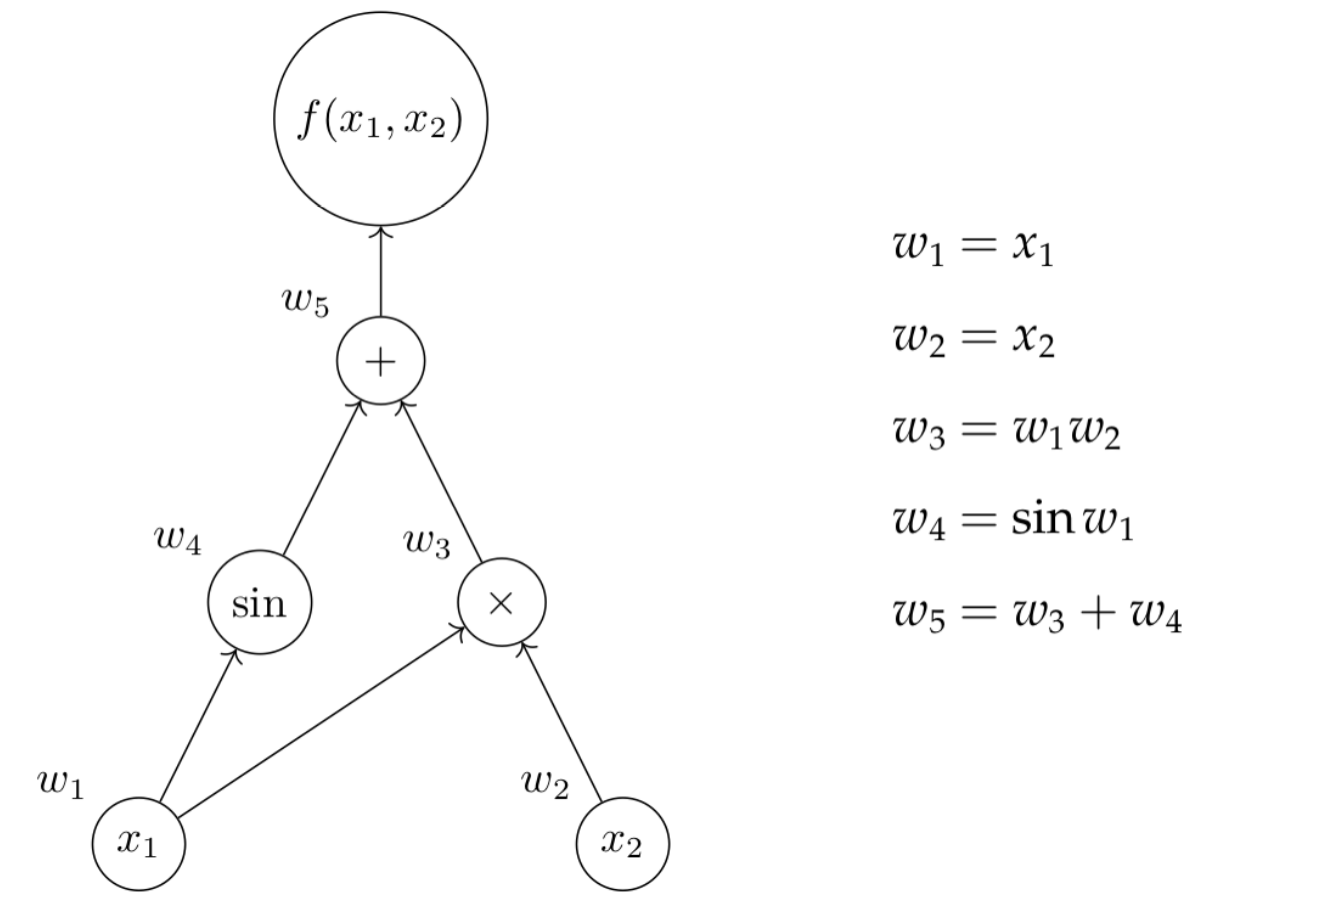
\includegraphics[scale=0.3]{1.png}
    \caption{函数微分计算结构图}
\end{figure}

\begin{figure}[h]
    \centering
    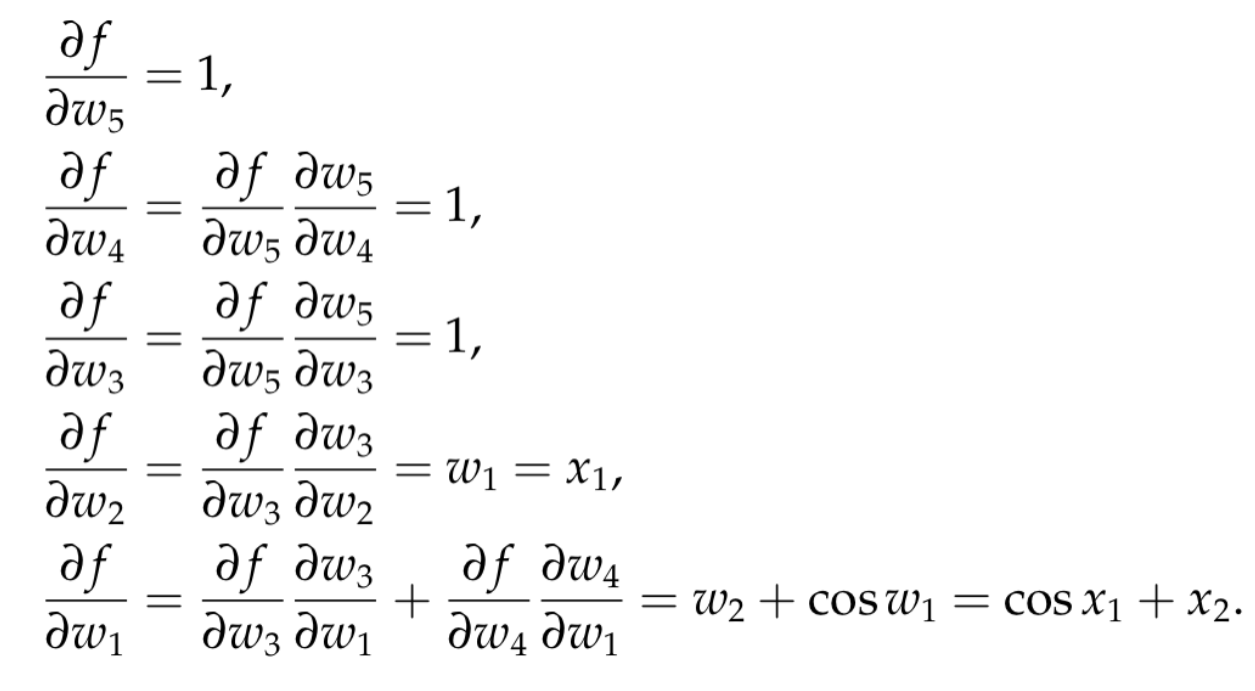
\includegraphics[scale=0.3]{2.png}
    \caption{函数微分计算过程图}
\end{figure}
以图1为例,前向梯度计算的过程先根据$w_1$和$w_2$的值来计算出$w_3$并得出对应的$\frac{\partial w_3}{\partial w_1}$以及$\frac{\partial w_3}{\partial w_2}$,通过链式法则依次求解。后向模式则是先根据$w_1$和$w_2$的值来计算出$w_3$,但是此时不求导,继续求后面的值,求完所有值后先求$\frac{\partial w_5}{\partial w_3}$以及$\frac{\partial w_5}{\partial w_4}$,从后往前求解。
后向模式的梯度计算复杂度更低,至多为函数值计算代价的5倍,自动微分基本上采用的都是后向的方法。
\section{广义实值函数}
将值域扩展,多了两个特殊的值$\pm\infty$。
\begin{definition}
    令$\overline{\mathbb {R}}$为$\mathbb {R} \cup \{ \pm\infty \}$为广义实值空间,则映射$f:\mathbb {R}^n \rightarrow \overline{\mathbb {R}} $为广义实值函数。
\end{definition}
\subsection{适当函数}
许多优化理论都是建立在适当函数的基础上的。适当函数定义为:至少有一个值不是正无穷且函数处处都不是负无穷。
\subsection{闭函数}
以下是一些定义。
下水平集:这是对于定义域来讲的,$C_a=\{ x|f(x) \le \alpha \}$。若$C_a$非空,那么全局最小点就一定落在$C_a$之中。
上方图:$epi \ f=\{(x,t) \in \mathbb{R}^{n+1}| f(x) \le t\} $
\begin{figure}[h]
    \centering
    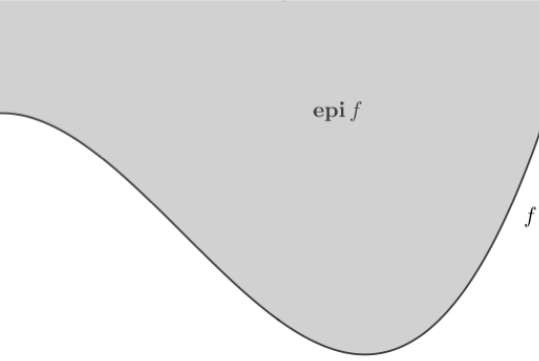
\includegraphics[scale=0.4]{3.png}
    \caption{上方图}
\end{figure}
闭函数与下半连续函数:这两个函数是等价的。
闭函数定义:设$f:\mathbb {R}^n \rightarrow \overline{\mathbb {R}} $为广义实值函数,若$epi$为闭集,则这个函数是闭函数。设广义实值函数$f:\mathbb {R}^n \rightarrow \overline{\mathbb {R}} $,若对任意的$x \in \mathbb{R}^n$有$$\lim\limits_{y \rightarrow x}inf \ f(y) \ge f(x) $$则$f(x) $为下半连续函数。其实就是在$x_0$ 处的邻域处,如果 $f(x_0) $减去一个正的微小值,从而可以恒小于该邻域的所有$f(x)$,则称在该间断点处有下半连续性。
\begin{figure}[h]
    \centering
    \subfigure[下半连续函数]{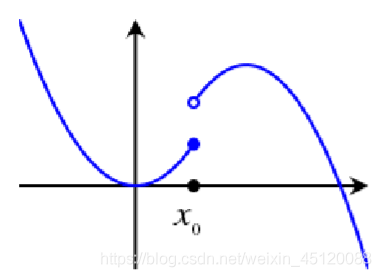
\includegraphics[scale=0.4]{4.png}
     }
    \subfigure[上半连续函数]{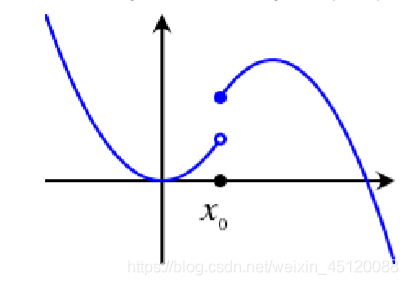
\includegraphics[scale=0.4]{5.png}
      }
\end{figure}
以下三个性质等价:闭函数、下半连续、任意下水平集都是闭集。

闭函数经过:加法、仿射、取上确界后依然是闭函数。
\section{凸集}
\begin{figure}[h]
    \centering
    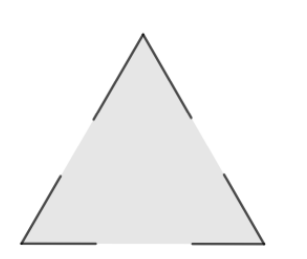
\includegraphics[width=5cm]{6.png}
    \caption{这个也是凸集}
\end{figure}
\section{凸函数}
\subsection{强凸函数}
定义为$f(x)$为凸函数且$\bigtriangledown ^2 f(x) \succeq mI ,m>0$。强凸性带来很多优秀的性质,比如二阶泰勒展开$f(y) \ge f(x)+\bigtriangledown f(x)^T (y-x)+\frac{m}{2}||y-x||^2_2$。
\subsection{凸函数判定定理}
方法1:先将函数限制在任意直线上,判定对应的一维函数是否是凸的。

定理:$f(x)$为凸函数当且仅当对任意的$x \in domf,v \in \mathbb{R}^n,g:\mathbb{R} \rightarrow \mathbb{R},$
$$g(t)=f(x+tv),\ {\rm dom}  \ g=\{t|x+tv \in {\rm dom} f\}$$是凸函数。

举个例子:判断$f(X)=-{\rm ln \ det}X$是凸函数。那么将这个函数限制在$X+tV$上,考虑一个函数$g(t)=f(X+tV)=-{\rm ln \ det}(X+tV)$,那么有$g(t)=-{\rm ln \ det}(X)-{\rm ln \ det}(1+tX^{-\frac{1}{2}}VX^{-\frac{1}{2}})=-{\rm ln \ det}(X)-\sum\limits_{i=1}^n ln(1+t \lambda_i)$,负对数函数很明显是凸的了。

注:这里应该是det符号里面可以随意换位,并且可以转置。

方法2:一阶条件,对于定义在凸集上的可微函数$f$,$f$是凸函数当且仅当$$f(y) \ge f(x)+\bigtriangledown f(x)^T(y-x)$$

方法3:梯度单调性,对于定义在凸集上的可微函数$f$,$f$是凸函数当且仅当$$(\bigtriangledown f(x)-\bigtriangledown f(y))^T(x-y) \ge 0$$
得到了相应的推论:$f$是严格凸函数当且仅当$$(\bigtriangledown f(x)-\bigtriangledown f(y))^T(x-y) > 0$$
$f$是m-强凸函数当且仅当$$(\bigtriangledown f(x)-\bigtriangledown f(y))^T(x-y) > m||x-y||^2$$

方法4:二阶条件,设$f$定义域为凸集且二阶连续可微函数,则$f$是凸函数当且仅当$$\bigtriangledown^2 f(x) \succeq 0 $$,如果是正定,那就是强凸函数。

方法5:设$f$定义域为凸集则$f$是凸函数当且仅当其上方图$epi f$为凸集
\subsection{保凸运算}
先留着,证明部分以后再看
%%%%%%%%%%%%%%%%%%%%%%%%%%%%%%%%%%%%%%%%%%%%%%%%%%%%%%%%%%%%%%%%%%%%%%%%%%%%%%%%%%%%%%%%%%%%%%%%%%%%%%%%%%%%%%%%%%%%%%%%%%%%%%%%%%%%%%%%%%%%%%%%%%%%%%%%%%%%%%%%%%%%%%%%
\section{共轭函数}
对于一个适当函数$f(x)$,它的共轭函数为$$f^*(y)=\sup\limits_{x \in dom f}\{y^Tx-f(x)\}$$
具有性质:Fenchel不等式
$$f(x)+f^*(y) \ge x^Ty $$
举例求一些函数的共轭:$f(x)=\frac{1}{2}x^TAx+b^Tx+c$,在强凸的情形下($A \succeq 0$),的共轭函数为$f^*(y)=\frac{1}{2}(y-b)^TA^{-1}(y-b)-c$。注:正定矩阵的逆的转置 等于 矩阵的转置的逆

再举个例子:凸集的示性函数
\begin{equation}
   I_c(x)=\left\{
    \begin{aligned}
        &0, &x \in C \\
        &+\infty , &x \notin C
    \end{aligned} 
   \right.
\end{equation}
对应的共轭函数就说$$f^*(y)=\sup\limits_{x \in dom f}\{y^Tx-I_C(x)\}=\sup\limits_{x \in dom f}y^Tx$$,所以这个又称为定义域的支撑函数

再举个例子:范数的共轭范数。若$$f(x)=||x||$$,共轭范数为
\begin{equation}
    I_c(x)=\left\{
     \begin{aligned}
         &0, &||y||_* \le 1 \\
         &+\infty ,&||y||_* > 1
     \end{aligned} 
    \right.
\end{equation}
\subsection{二次共轭函数}
已知$$f^*(y)=\sup\limits_{x \in dom f}\{y^Tx-f(x)\}$$,那么二次共轭函数就是
$$f^{**}(x)=\sup\limits_{y \in dom f^*}\{x^Ty-f^*(y)\}$$
这个二次共轭函数一定是个凸函数,并且有$f^{**}(x) \le f(x)$或者等价的说$epi f \subseteq epi f^**$,等号在原函数是凸的时候成立。
%%%%%%%%%%%%%%%%%%%%%%%%%%%%%%%%%%%%%%%%%%%%%%%%%%%%%%%%%%%%%%%%%%%%%%%%%%%%%%%%%%%%%%%%%%%%%%%%%%%%%%%%%%%%%%%%%%%%%%%%%%%%%%%%%%%%%%%%%%%%%%%%%%%%%%%%%%%%%%%%%%%%%%%%
\section{次梯度}
\subsection{次梯度的定义}
设$f$为适当凸函数,$x$为定义域$dom f$中的一点,若向量$g \in \mathbb{R}^n$满足
$$f(y) \ge f(X)+g^T(y-x) ,\forall y \in domf$$
那么$g$就是在函数$f$处的一个次梯度。进一步的,称集合$$\partial f(x) =\{g|g \in \mathbb{R}^n,f(y) \ge f(x)+g^T(y-x), \ \forall y \in domf\}$$为$f$在$x$处的次微分。
\begin{figure}
    \centering
    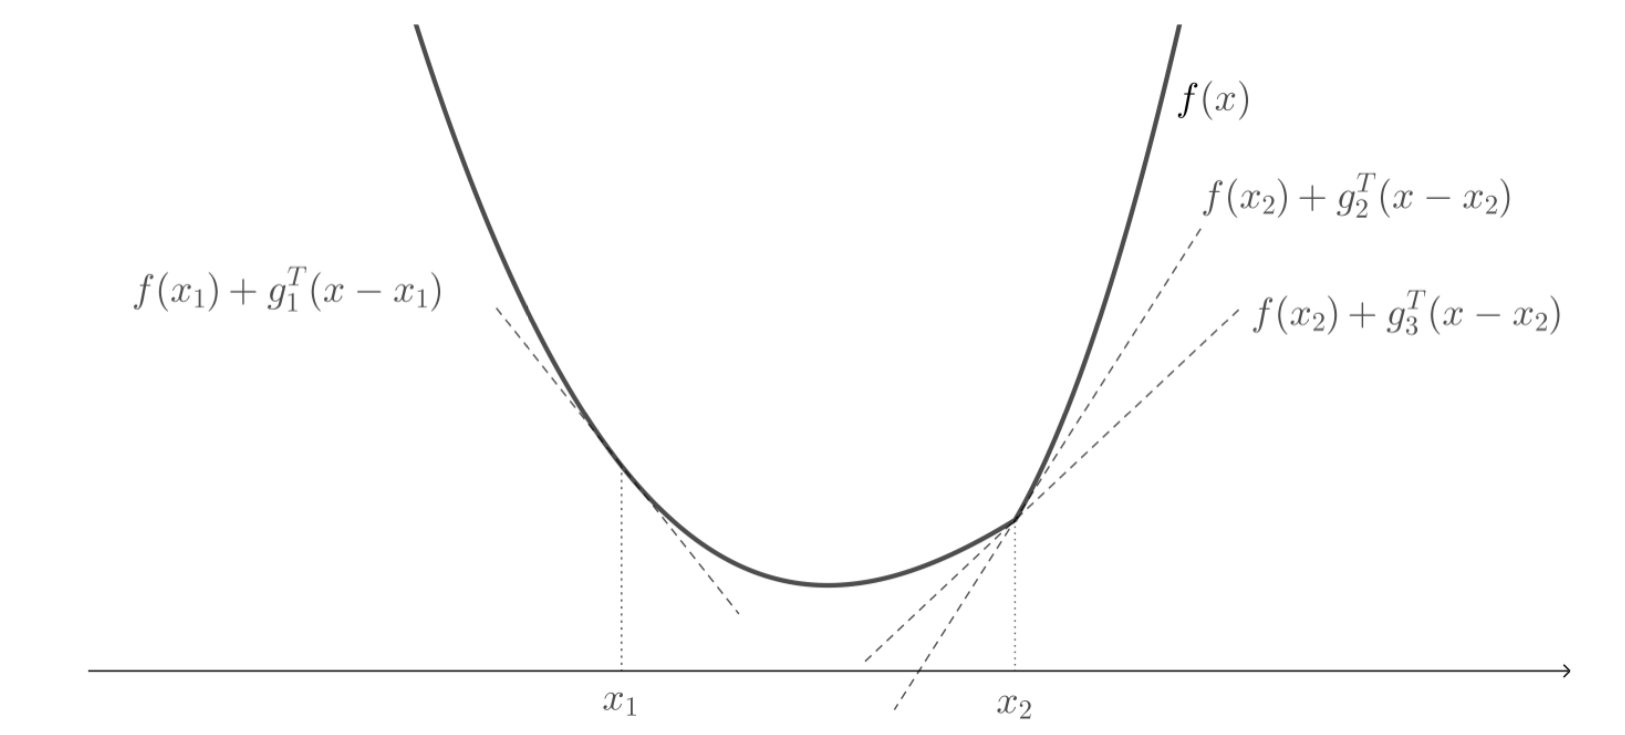
\includegraphics[width=9cm]{7.png}
    \caption{f(x)的次梯度}
\end{figure}
也可以在图5中看到,部分点是有一个次梯度,部分点是有多个。从次梯度的定义中也可以得出,如果$g$是$f$在$x_0$处的次梯度,那么函数$$l(x)=f(x_0)+g^T(x-x_0)$$为凸函数$f(x)$的一个全局下界。同时也可以推导处上方图在这个点的支撑超平面。

次梯度的存在性。$f$为适当凸函数,如果点$x_0$是定义域的内点(也就是$x_0 \in {\rm intdom} f$),那么就存在次梯度。

次微分的计算。以$f(x)=||x||_2$为例,求在$x=0$处的次微分。根据定义得到
$f(y)-0 \ge g^T(y-0)$,
也就是$||y||_2 \ge g^T(y)$
因此$||g||_2 \le 1$就是次微分。
再带入$||g||_2 \ge 1$发现不符合,求解结束。

\subsection{次梯度的性质}
定理:设$f$是凸函数,那么$\partial f(x)$就有以下性质。

1.对于任何$x \in domf$,那么$\partial f(x)$就是一个闭凸集。如果$x \in intdomf$,那么$\partial f(x)$就说非空的有界集。

2.如果$f(x)$在$x_0 \in intdomf$处可微,那么次梯度就是梯度,$\partial f(x)=\bigtriangledown f(X)$。

3.次梯度的单调性。设$f: \mathbb{R}^n \rightarrow \mathbb{R}$,且$(u-v)^T(x-y) \ge 0$,其中$u \in \partial f(x),v \in \partial f(y)$

4.某种程度上的连续性。如果,$x^k \Rightarrow \overline{x}$且$g^k \Rightarrow \overline{g},g^k \in \partial f(x^k)$那么就会有$\overline{g} \in \partial f(\overline{x})$
这个相当于要求了$g^k$是闭集,也等价于$\partial f(x)$的图像${(x,g)|g \in \partial f(x),x \in domf}$是闭集。
\subsection{凸函数的方向导数}
设$f$为适当函数,给定点$x_0$以及方向$d \in \mathbb{R}^n$,方向导数定义为
$$\lim\limits_{t \downarrow 0} \phi (t)=
\lim\limits_{t \downarrow 0} \frac{f(x_0+td)-f(x_0)}{t}
$$
这和之前计算矩阵的梯度十分相似啊。$t \downarrow 0$表示$t$单调下降趋于0。凸函数是一个单调不减的函数,所以$lim$也可以换成下确界$inf$。
那么,方向导数的定义还可以更新为
$$
\partial f(x_0;d)=\inf\limits_{t>0}\frac{f(x_0+td)-f(x_0)}{t}
$$

命题:只要$f(x)$是凸函数,且$x_0 \in intdom f$,则对任意$d \in \mathbb{R}^n$,梯度$\partial f(x_0;d)$是有限的。并且$\partial f(x_0;d)=\max\limits_{g \in \partial f(x_0)}g^Td$,$\partial f(x_0;d)=\sup\limits_{g \in \partial f(x_0)}g^Td$。
\subsection{次梯度计算规则}
可微凸函数,次梯度就是梯度。
凸函数的非负线性组合,次微分也是相应组合。比如$f=a_1f_1+a_2f_2$,那么$\partial f=a_1\partial f_1+a_2\partial f_2$(仅指内部的点)。
线性变量的替换,比如$f(x)=h(Ax+b)$,那么次微分之间的关系就是$\partial f(x)=A^T\partial h(Ax+b), \forall x \in intdomf$。

函数族的上确界。比如说$f(x)=\max\{f_1(x),f_2(x),\dots,f_m(x)\}$,那么对应的梯度就是
$\partial f(x_0)=conv \partial \cup_{i \in I(x_0)}f_i(x_0)$
其实就是各个点的次微分的组合。举个例子,
\begin{figure}[h]
    \centering
    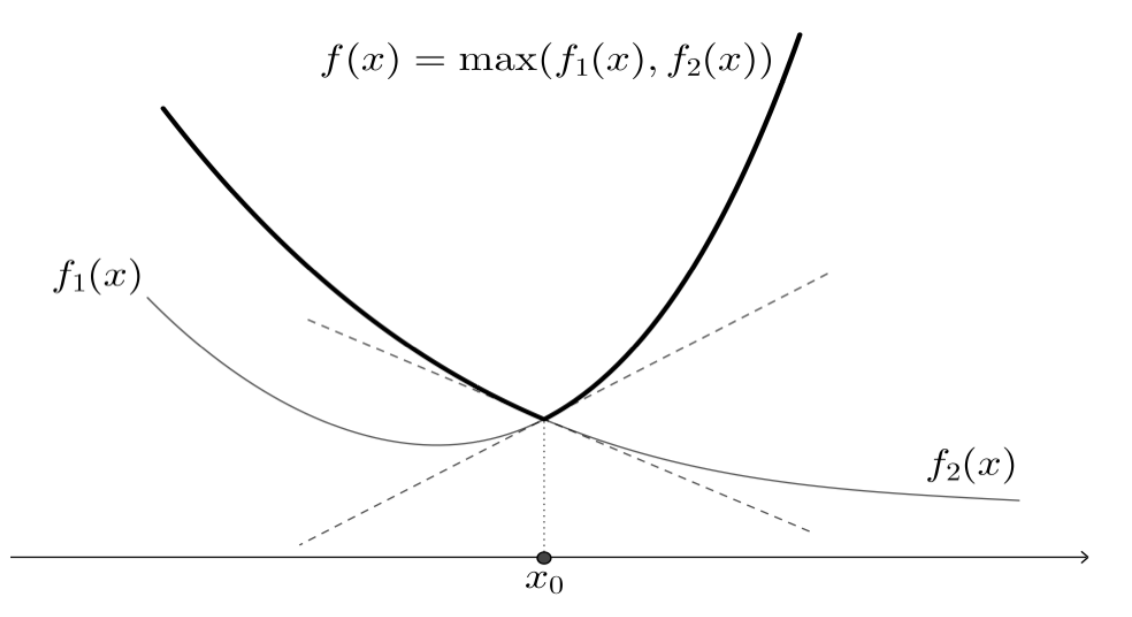
\includegraphics[width=7cm]{8.png}
    \caption{两个函数的最大值}
\end{figure}
那么在$x=x_0$处,$\partial f(x)=\{v|v=t\bigtriangledown f_1(x)+(1-t)\bigtriangledown f_2(x)\}$,对于$x<x_0,\partial f(x)=\{\bigtriangledown f_2(x)\}$,对于$x>x_0,\partial f(x)=\{\bigtriangledown f_2(x)\}$

看到72页,到后面75页以后再来看。
\end{document}